\documentclass[ignorenonframetext]{beamer}
%\usetheme{Boadilla}
\usetheme{PaloAlto}
%\usetheme{Berlin}
%\usecolor{}

\mode<presentation>

\usepackage{minted}


\usepackage{fontspec}
\setmainfont{Linux Libertine O}

\usepackage{tikz}

\usepackage[english,french]{babel}

\institute{École nationale des chartes | Paris, Sciences \& Lettres}

\title{Introduction}
\subtitle{Atelier \textit{Humanités numériques}}
\author{Jean-Baptiste Camps}
\date[Madrid, 9 oct. 2018]{Casa de Velázquez\\ Madrid, 9 octobre 2018}

\makeatletter 
         
        \AtBeginSection[]{% 
        \begin{frame}{Plan}%
        \small
        \tableofcontents[currentsection]%
        \end{frame} }

        %\AtBeginSubsection[]{% 
	%\begin{frame}{Plan}%
	%\small
	%\tableofcontents[currentsection,currentsubsection]%
%\end{frame} }


\makeatother 
    
    
\begin{document}

\frame{\maketitle}

%\frontmatter 
  

%\mainmatter 


% 1h, on peut compter entre 40 et 50 de slides
% % 1. Définition / historique / mon approche
% % 2. Collecter et structurer les données
% % % 2.1 Interroger et collecter des données depuis des entrepôts (API)
% % % (questions juridiques)
% % % 2.2 Produire ses données
% % %     - acquisition des données de base
% % %     - nettoyage
% % %     - enrichissement
% % % 2.3 Structuration des données, standards
% % %      - questions de formats
% % %      - questions de référentiels
% % 3. Interroger et Analyser les données
% % % 3.1 Outils d'interrogation
% % % 3.2 Méthodes quantitatives: des corrélations à la modélisation
% % % 3.3 Quelques outils particuliers des sciences sociales (réseaux, SIG, …)




\section{Définition?}

\begin{frame}{Faut-il vraiment définir les humanités numériques?}

	\begin{columns}
	\begin{column}{0.45\textwidth}
		\begin{itemize}
			\item interdiscipline?
			\item transdiscipline?
			\item science auxiliaire?
			\item approche méthodologique?
			\item courant historiographique? Mode?
			\item source de financement?
			\item ``cheval de Troie néolibéral''?
		\end{itemize}
	\end{column}
	\begin{column}{0.45\textwidth}
		Dans les humanités numériques francophones, beaucoup de temps a été pris, dans les années 2010, par la question de la \alert{définition} des humanités numériques…
	\end{column}
\end{columns}

\end{frame}

\begin{frame}{Une définition et une distinction}
	
	\begin{block}{Définition de travail}
		Mise en œuvre de méthodes numériques en sciences humaines.
	\end{block}
	
	\begin{block}{Ne pas confondre}
		\begin{description}
			\item[humanités numériques] numérique \alert{en} sciences humaines;
			\item[``études numériques''] numérique comme \alert{objet d'étude} des sciences humaines (y compris de manière très traditionnelle); \textit{digital studies.}
		\end{description}
	\end{block}
	
\end{frame}

\subsection{Survol historique}

\begin{frame}<1>[label=chrono]
	
	\frametitle{Quelques dates: chronologie sélective et personnelle}

	\begin{description}
		\only<1-2>{
			\item[1941-9] Robert Busa conçoit le projet d'\textit{Index Thomisticus} appuyé sur des machines. En 1949, il convainc Thomas J. Watson, fondateur d'IBM;
			\item[1946] A.D. Booth entreprend la conception d'une ``traductrice automatique'';
		}
		\only<2>{
			\item[1966] création de la revue \textit{Computers and the Humanities};
			\item[1967] Charles Muller soutient à Strasbourg sa thèse \textit{Étude de statistique lexicale: le vocabulaire du théâtre de Pierre Corneille};
			\item[1968] Dom Froger publie \textit{La Critique des textes et son automatisation};
		}
	\only<3-4>{
		\item[1980-…] le terme d'\textit{Humanities computing} se répand, avec la création de centres dans les univ. anglo-saxonnes;
		\item[1982] mise sur le marché du Commodore 64;
		\item[1987] établissement de la \textit{Text Encoding Initiative};
		\item[1996] spécification \textsc{xml};
	}
	\only<4>{
	\item[1989-1993] Tim Berners-Lee propose et mène la création du Web (au CERN);
	\item[2004] Parution d'\textit{A Companion to Digital Humanities};
	\item[2007] Jim Gray propose le concept de \textit{data science}.
}
		
	\end{description}
	
\end{frame}

\begin{frame}
\frametitle{Années 1940-1960}
\framesubtitle{Les jésuites, les bénédictins et les autres}

Un premier projet d'ampleur: l'indexation et la lemmatisation de l'œuvre de saint Thomas d'Aquin.

%N.B.: à cette époque, les programmeurs sont très souvent des programmeuses.

\begin{columns}
	\begin{column}{0.5\textwidth}
		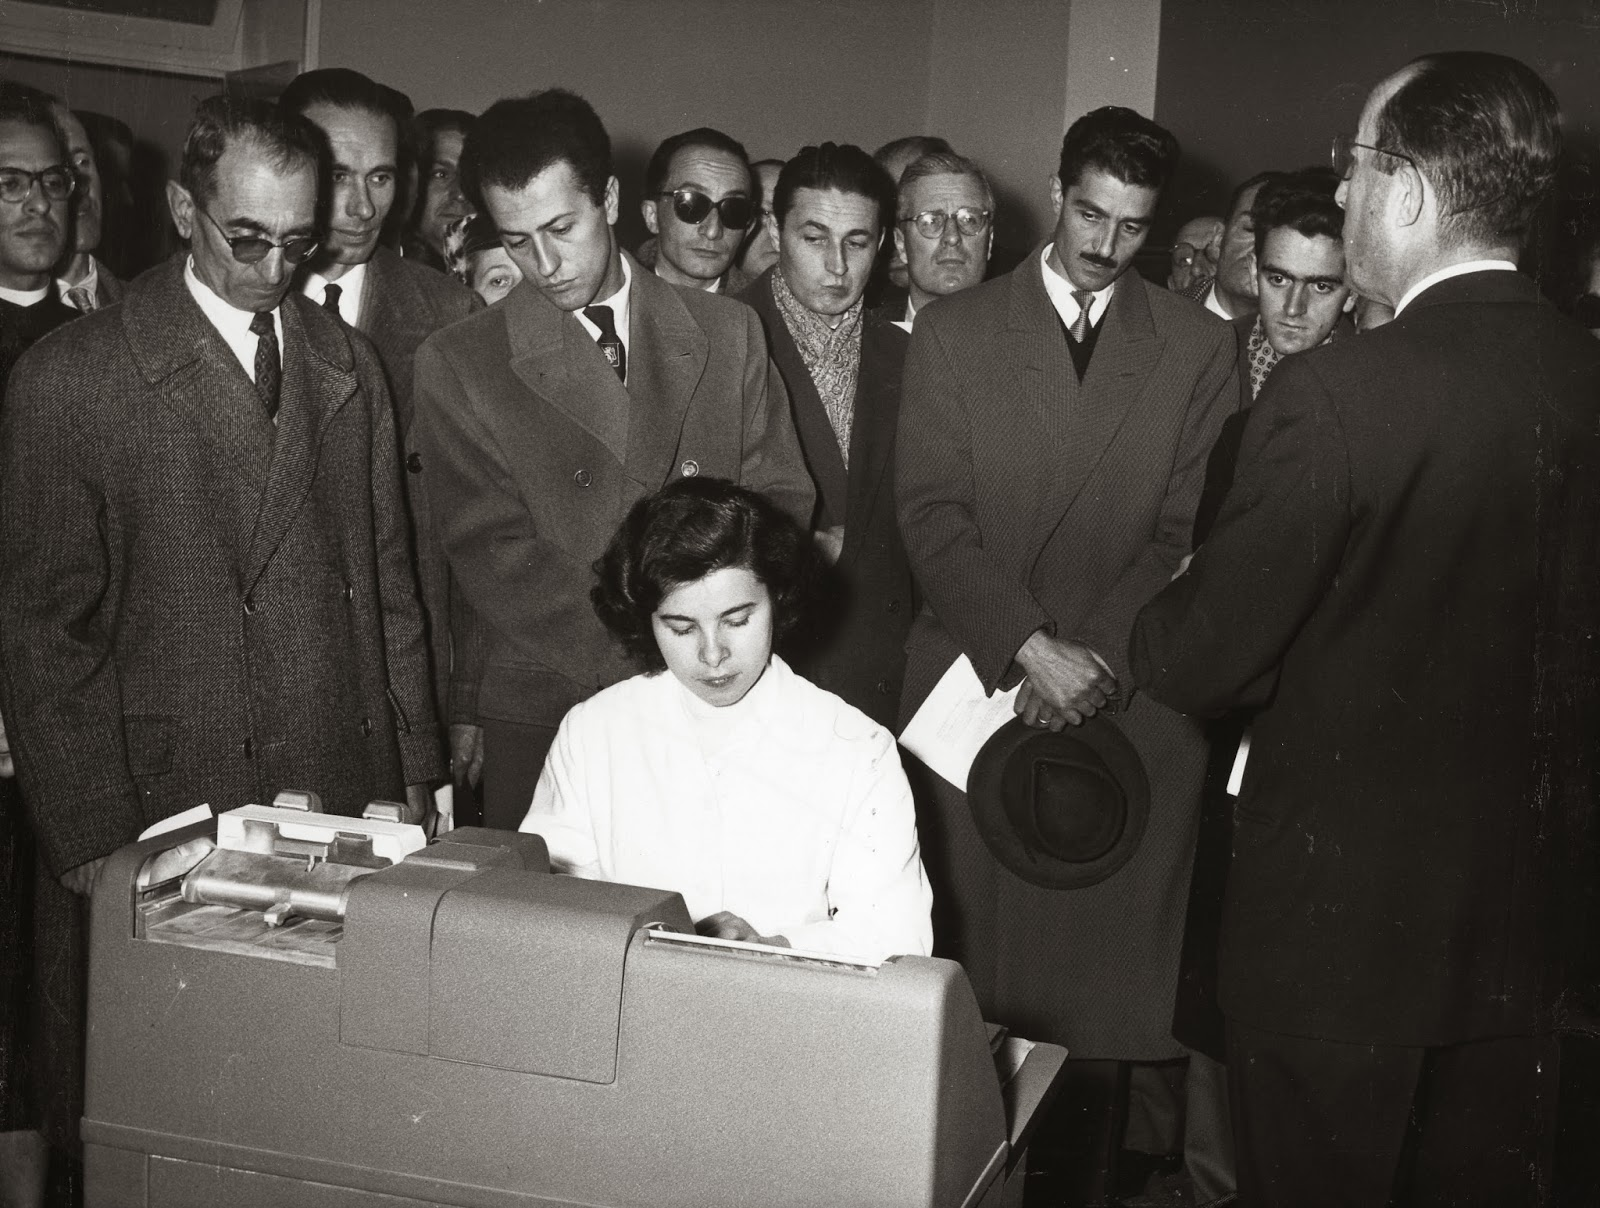
\includegraphics[width=\textwidth]{img/livia_canestrano_0085.jpg}
		
	\end{column}
	\begin{column}{0.5\textwidth}
		
		
		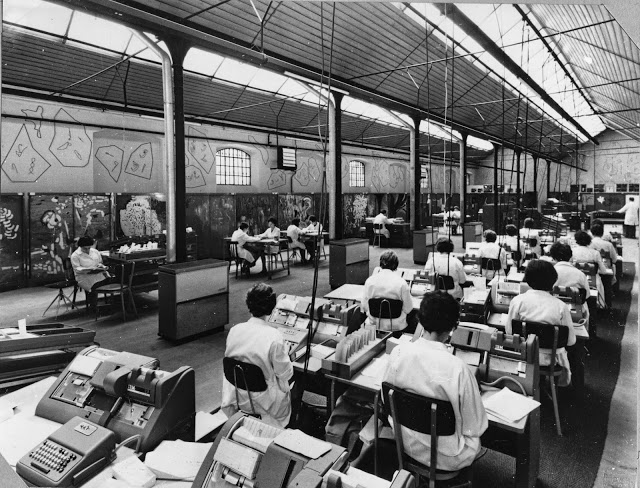
\includegraphics[width=\textwidth]{img/thomisticus_0613.jpg}
	\end{column}
\end{columns}

{\footnotesize
	\textit{Livia Canestrano au travail sur l'Index Thomisticus (gauche), l'atelier de Gallarate (droite); années 1950-1960; arch. R. Busa}
	
	CC-BY-NC, \url{http://melissaterras.blogspot.com/2013/10/for-ada-lovelace-day-father-busas.html}
}

\end{frame}

\begin{frame}[shrink]
\frametitle{Années 1940-1960}
\framesubtitle{Les jésuites, les bénédictins et les autres}

\begin{block}{Dom J. Froger, La Critique des textes et son automatisation, 1968.}
	
	Depuis vingt ans, exactement depuis qu'en 1946 A.D. Booth entreprit de construire une traductrice automatique, les philologues utilisent de plus en plus fréquemment les ordinateurs : au mois de mai de cette année une revue spécialisée, \textit{Computers and the Humanities}, énumère cent vingt programmes en cours d'exécution, et l'énumération n'est pas exhaustive.
	
	La plupart de ces travaux sont, en dernière analyse, des \textit{index verborum} (...) on peut considérer l'ordinateur comme l'instrument par excellence de tous les travaux qui relèvent plus ou moins directement de la lexicographie. (...)
	
	Il est maintenant \alert{courant d'« automatiser » les recherches philologiques ou littéraires, et d'utiliser la machine électronique ou mécanographique pour des études lexicographiques ou stylistiques ; ces procédés ont déjà été employés pour aider à la critique conjecturale, et par exemple combler les lacunes des manuscrits de la mer Morte}
	
	En 1960-61, sous la direction de Mme Poyen, deux \og{}programmes\fg{} destinés à l'ordinateur Gamma ET Bull ont été établis : l'un (...) pour la collation, l'autre (...) pour la recherche de l'enchaînement des manuscrits d'après leurs variantes.
\end{block}


\end{frame}

\againframe<2>{chrono}

% Développement du TAL
% Développement de l'histoire quantitative
% 

\begin{frame}
\frametitle{Années 1960-1970}
\framesubtitle{Histoire, linguistique, philologie, lexicographie… \emph{quantitatives}}


\begin{block}{Emmanuel Le Roy Ladurie (1968)}
	L'historien de demain sera programmeur ou il ne sera pas.
\end{block}


\includegraphics[width=\textwidth]{img/ahess_0395-2649_1971_num_26_2_T1_0478_0001_1.png}

{\footnotesize %
Micheline Baulant, \og{}Le salaire des ouvriers du bâtiment à Paris, de 1400 à 1726\fg{}, \textit{Annales} (1971).
}

\end{frame}

% Recul du quantitatif (années 1980)

\againframe<3>{chrono}

\begin{frame}
\frametitle{Années 1980-1990}
\framesubtitle{Arrivée du micro-ordinateur | Recul du quantitatif}

\begin{columns}
	\begin{column}{0.45\textwidth}
		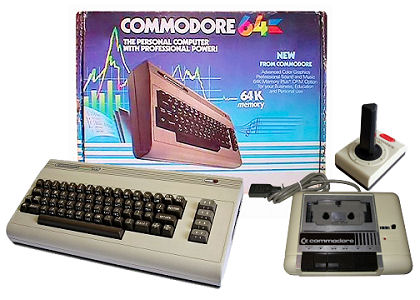
\includegraphics[width=\textwidth]{img/commodore-64-system.jpg}
	\end{column}
	\begin{column}{0.45\textwidth}
		Il est de bon ton, pour certains, de jouer aux princes de l'intelligence en dédaignant superbement, comme des contingences subalternes, des mesquineries de tâcheron, les exigences de la rigueur et les contraintes de la quantification \\
	(Antoine Prost, \textit{Douze leçons sur l'histoire}, 1996)
	\end{column}
\end{columns}

\end{frame}

\begin{frame}
\frametitle{Années 1980-1990}
\framesubtitle{Structuration des données et corpus textuels}


\begin{block}{Les Principes de Poughkeepsie (1987)}

Proposer des \textit{Guidelines} pour:

\begin{itemize}
	\item[1] provide a standard format for data interchange in humanities research.
	\item[2] suggest principles for the encoding of texts in the same format.
	\item[3] define a recommended syntax for the format, a metalanguage for the description of text-encoding schemes, describe the new format and representative existing schemes both in that metalanguage and in prose;
	\item[4] propose sets of coding conventions suited for various applications.
	\item[5] include a minimal set of conventions for encoding new texts in the format.
\end{itemize} 
\end{block}

\end{frame}

\againframe<4>{chrono}
%TODO
%\begin{frame}
%\frametitle{Années 2000-2010}
%\framesubtitle{\textit{Digital humanities}, web et \textit{Data deluge}}
%
%\begin{columns}
%	\begin{column}{0.45\textwidth}
%		
%	\end{column}
%	\begin{column}{0.45\textwidth}
%		
%	\end{column}
%\end{columns}
%
%\end{frame}

\begin{frame}
\frametitle{Années 2000-2010}
\framesubtitle{De l'\textit{Humanities Computing} aux \textit{Digital Humanities}}

\begin{itemize}
	\item Terme de \textit{Digital Humanities} créé par Johanna Drucker, John Unsworth et Jerome McGann, à la fin des années 1990
	\item remplacer le terme d’« Humanities Computing », « too closely associated with computing support services »
	\item Ce changement devait signifier que ce champ « had emerged from the low-
	prestige status of a support service into a genuinely intellectual endeavour with its own professional practices, rigorous standards, and exciting theoretical explorations.
\end{itemize}

\end{frame}


\begin{frame}{Et maintenant?}

\begin{columns}
	\begin{column}{0.45\textwidth}
		\Large Humanités digitales (?)
		
		\centering
		
		
\includegraphics[width=0.7\textwidth]{img/manicule07.jpg}
	\end{column}
	\begin{column}{0.45\textwidth}
		\Large Humanités computationnelles ou tournées vers les données
	\end{column}
\end{columns}

\end{frame}

% des humanités numériques aux sciences humaines computationnelles ou tournées vers les données

\subsection{Des humanités numériques au computationnel et à la science des données}

\begin{frame}{Des humanités numériques, computationnelles ou intensives en données?}

%Graphique de Stanford
\begin{columns}
	\begin{column}{0.65\textwidth}
		%\begin{center}
			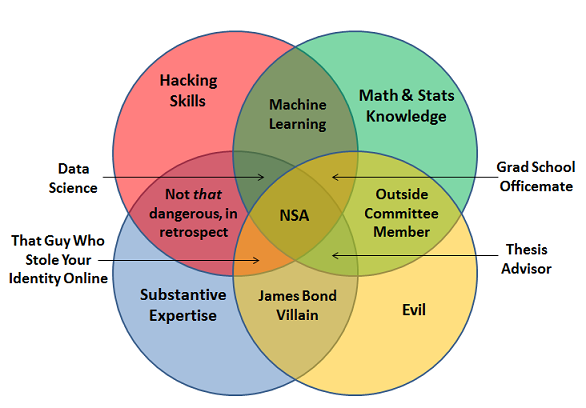
\includegraphics[width=\textwidth]{img/VennDiagram2.png}
		%\end{center}
		
		%{\tiny Source: Joel Grus, « Post-Prism Data Science Venn Diagram », 9 juin 2013, \url{http://joelgrus.com/2013/06/09/post-prism-data-science-venn-diagram/}, repris par Elijah Meeks, \og{}Digital Humanities and Data Science\fg{}, \textit{Stanford Digital Humanities}, 2014, \url{https://digitalhumanities.stanford.edu/digital-humanities-and-data-science}.}
	\end{column}
	\begin{column}{0.4\textwidth}
		%\begin{block}
		\alert{4 paradigmes de la recherche scientifique selon Jim Gray}
			\begin{itemize}
				\item \textbf{expérimentale}
				\item \textbf{théorique}
				\item \textbf{computationnelle}
				\item \textbf{intensive en données}
			\end{itemize}
		%\end{block}
	\end{column}
\end{columns}

\end{frame}


\section{Collecte et structuration des données}

% % 2. Collecter et structurer les données
% % % 2.1 Interroger et collecter des données depuis des entrepôts (API)
% % % (questions juridiques)

\subsection{Interroger et collecter des données depuis des entrepôts (API)}

% Sources de données (institutions, dépôts de données de recherche, projets,…).

\begin{frame}{Sources de données}

		\begin{block}{Sources institutionnelles}
			\begin{itemize}
				\item bibliothèques numériques: Gallica, E-Codices, …
				\item portails d'institutions patrimoniales: data.bnf,…
				\item entrepôts de données de la recherche: Zenodo, …
				\item portails universitaires ou de laboratoires: University of Oxford Text Archive, ressources de l'IRHT… 
				\item projets divers et variés: sites des projets, s'ils sont encore maintenus; \textit{Wayback Machine sinon…}
			\end{itemize}
		\end{block}
	
	\begin{block}{Autres sources}
		\begin{itemize}
			\item données produites par une communauté (e.g. Wikidata…)
			\item corpus et bases de données payantes (Brepols, Garnier…);
			\item entrepôts de code source: Github, …
		\end{itemize}
	\end{block}

\end{frame}

\begin{frame}{Questions juridiques}


			\begin{block}{Droits patrimoniaux et domaine public}
				Droit d'auteur: naît d'un acte original de création.\\
				Cas général: entrée dans le domaine public \\
				70 ans après la mort de l'auteur.
			\end{block}
			\begin{block}{Copyfraud}
				(Ré)éditer une œuvre du domaine public \textit{ne crée} pas de nouveau droit.\\
				Se méfier de certaines indications sur les sites commerciaux, nulles et non avenues.
			\end{block}
	
\end{frame}

\begin{frame}{Questions juridiques}

		\begin{block}{Licence}
			\begin{itemize}
				\item libre?
				\item licence similaire aux œuvres dérivées?
				\item réutilisation commerciale?
				\item œuvres dérivées?
			\end{itemize}
		\end{block}
		\begin{block}{Exception du droit à la fouille de données}
			loi du 7 octobre 2016 « Pour une République numérique »\\
			Exception au droit d'auteur:\\
			\textit{ Les copies ou reproductions numériques réalisées à partir d'une source licite, en vue de l'exploration de textes et de données incluses ou associées aux écrits scientifiques pour les besoins de la recherche publique, à l'exclusion de toute finalité commerciale}		 
			%https://ethiquedroit.hypotheses.org/1528
		\end{block}

\end{frame}

\begin{frame}[fragile]
\frametitle{Comment récupérer les données?}


\begin{tikzpicture}

\node[draw, rectangle, rounded corners=3pt] (P) at (6,6)
{La possibilité a-t-elle été prévue?};%

\node[draw, rectangle, rounded corners=3pt] (N) at (8.5,4)
{Compliquée?};%

\node[draw, rectangle, rounded corners=3pt] (S) at (7,1)
{script simple};%

\node[draw, rectangle, rounded corners=3pt] (T) at (10,1)
{script ``avancé''};%


\node[draw, rectangle, rounded corners=3pt] (O) at (3.5,4)
{Quel besoin?};%

\node[draw, rectangle, rounded corners=3pt] (A) at (2,1)
{csv};%

\node[draw, rectangle, rounded corners=3pt] (B) at (3.5,1)
{API};%

\node[draw, rectangle, rounded corners=3pt] (C) at (5,1)
{entrepôt};%

\draw[->,>=latex] (P) -- (N) node[midway,sloped,above] {non}; 
\draw[->,>=latex] (P) -- (O) node[midway,sloped,above] {oui}; 
\draw[->,>=latex] (N) -- (S) node[midway,sloped,above] {non}; 
\draw[->,>=latex] (N) -- (T) node[midway,sloped,above] {oui}; 
\draw[->,>=latex] (O) -- (A) node[midway,sloped,above] {export simple}; 
\draw[->,>=latex] (O) -- (B) node[midway,sloped,above] {requête}; 
\draw[->,>=latex] (O) -- (C) node[midway,sloped,above] {sources}; 

\end{tikzpicture}


\end{frame}

% Définir ce qu'est une API

\begin{frame}{Les APIs}
	%Capture d'écran site APIs BNF
	%Définition
	
		\begin{columns}
		\begin{column}{0.5\textwidth}
			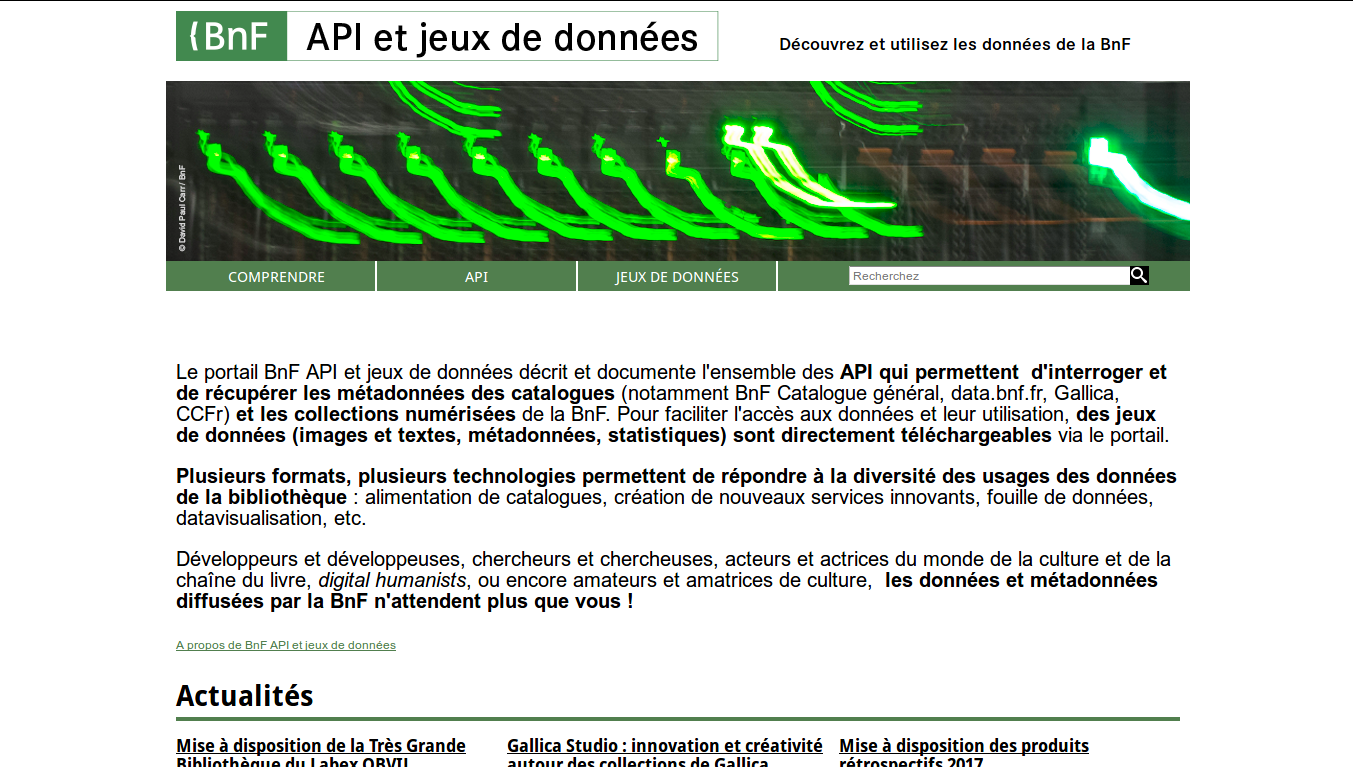
\includegraphics[width=\textwidth]{img/API_BnF.png}
			{\footnotesize \textit{Le site api.bnf.fr}}
		\end{column}
		\begin{column}{0.50\textwidth}
			\begin{block}{Application Programming Interface}
				Un ensemble de méthodes et d'outils prédéfinis,\\
				qui peuvent servir de base à la construction de requêtes ou de programmes.\\
				
				Un peu l'équivalent pour programmeur de l'interface graphique pour l'utilisateur.
			\end{block}
		\end{column}
	\end{columns}

\end{frame}


% Exemple de IIIF
% Exemple de CTS/DTS?


\begin{frame}{Un exemple d'API: IIIF}

% Documentation, et explication
% Ex. de requête Gallica

\begin{block}{} \footnotesize
	\texttt{https://gallica.bnf.fr/iiif/ark:/12148/btv1b9045910f/f0/full/600/180/native.png}\\
	\texttt{{scheme}://{server}{/prefix}/{identifier}/{region}/{size}/{rotation}/{quality}.{format}.}
\end{block}

\begin{center}
	
\includegraphics[width=0.7\textwidth]{img/Casa.png}
\end{center}

\end{frame}

\begin{frame}[fragile]

\frametitle{Un autre exemple: Canonical Text Services}

% Documentation, et explication
% Ex. de requête Gallica

\begin{block}{} \small

\href{http://dev.chartes.psl.eu/elec/geste/api/cts?request=GetPassage&urn=urn:cts:froLit:geste.jns11095.transcr_Otin_B:1-10}{\texttt{http://dev.chartes.psl.eu/elec/geste/api/cts?request=GetPassage\&urn=urn:cts:froLit:geste.jns11095.transcr\_Otin\_B:1-10}}
	
\end{block}

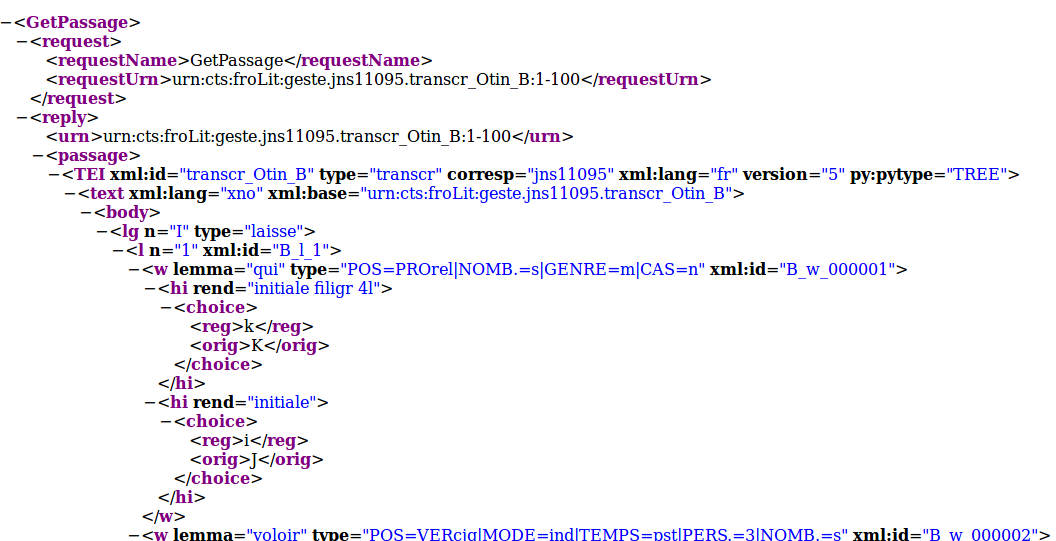
\includegraphics[width=\textwidth]{img/NemoAPI.png}

\end{frame}

\subsection{Construire ses données}

% % % 2.2 Produire ses données
% % %     - acquisition des données de base
% % %     - nettoyage
% % %     - enrichissement


\begin{frame}{Acquisition des données}

Si les données n'existent pas sous forme numérique, il faut les construire soi-même.
	
	% Texte (OCR)
	% Image -> reconnaissance de motifs
	% 
	
	
		\begin{block}{Acquisition de données textuelles}
			\begin{itemize}
				\item imprimées: OCR (Tesseract, …);
				\item manuscrites: transcription, HTR (Transkribus, OCRopy,…);
			\end{itemize}
		\end{block}
	
	\begin{block}{Nettoyage / Post-correction}
		Des logiciels de post-correction existent,\\
		fondés sur des dictionnaires, des règles, des corrections en série.
		\begin{itemize}
			\item Antidote (payant) pour les langues contemporaines;
			\item PoCoTo (libre, dév. par le CISOCR group, Munich): permet de 
			créer des modèles pour les anciens états de langue; \url{https://github.com/cisocrgroup/PoCoTo}.
		\end{itemize}
	\end{block}
	
\end{frame}

\begin{frame}{Nettoyer ou fusionner des jeux de données}

% Outils comme Dataïku ou OpenRefine

Des outils permettent de faciliter le nettoyage ou la fusion de jeux de données originellement mal structurés ou distincts, ex. Dataiku, OpenRefine,…

\begin{center}
	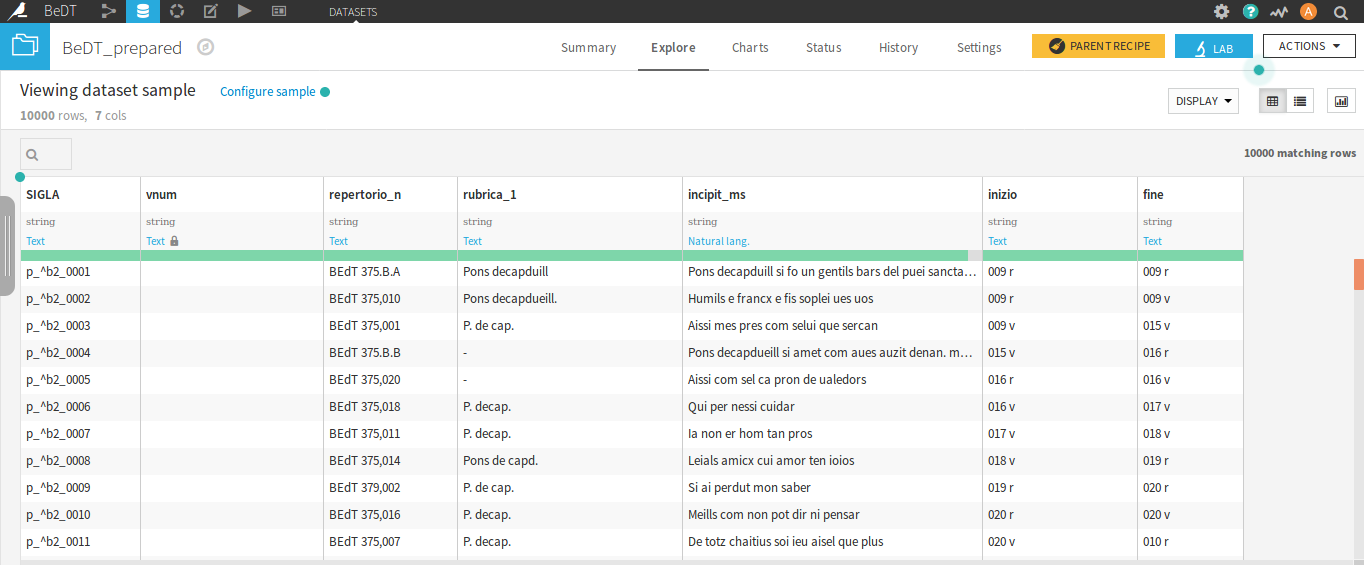
\includegraphics[width=0.8\textwidth]{img/Dataiku.png}
\end{center}

\end{frame}

\begin{frame}{Enrichissement des données}

Quelques exemples d'enrichissements pouvant recevoir le soutient de méthodes computationnelles…

% Lemmatisation + post-correction
\begin{block}{Lemmatisation}
Des lemmatiseurs fondés sur
	\begin{itemize}
		\item des lexiques de forme, ex. TreeTagger;
		\item des modèles d'apprentissage machine, ex. Lemming, Pandora,…
	\end{itemize}
Des outils de post-correction, ex. Pandora Post-Correction Editor (\url{http://dev.chartes.psl.eu/ppa/}).
\end{block}

% Reconnaissance des entités nommées (SAM), Recogito, …

\begin{block}{Reconnaissance des entités nommées}
	\begin{itemize}
		\item SEM, \url{http://apps.lattice.cnrs.fr/sem/};
		\item Recogito, \url{https://recogito.pelagios.org} (\href{https://recogito.pelagios.org/document/qgehu36kmc3bdz/part/1/edit}{ex.}).
	\end{itemize}
\end{block}


\end{frame}

% % % 2.3 Structuration des données, standards
% % %      - questions de formats
% % %      - questions de référentiels

\subsection{Structuration des données}

%interopérabilité, pérennité, FAIR principles

\begin{frame}{\textsc{Fair} Data}
%Cf. les principes soutenus par les États et agences de recherche (CE, ERC,…)
\begin{center}
	
\includegraphics[width=0.6\textwidth]{img/FAIR_data_principles.jpg}
	
	{\footnotesize (Img. SangyaPundir CC BY-SA 4.0)}%, \url{https://commons.wikimedia.org/w/index.php?curid=53414062}}
\end{center}

\begin{columns}[T]
	\begin{column}{0.5\textwidth}
		\begin{itemize}
			\item \textit{Findable}: données doivent être faciles à trouver en ligne, y compris sur le long terme (archivage pérenne);% provinding persistents identifier. 
			\item \textit{Accessible}: format ouvert, libre, documenté et compréhensible;
		\end{itemize}
	\end{column}
	\begin{column}{0.5\textwidth}
		\begin{itemize}
			\item \textit{Interoperable}: pas enfermées dans un logiciel propriétaire; standards, intégrité des données, documentation;
			\item \textit{Reusable}: données ouvertes, réutilisables  (légalement, techniquement,…).
		\end{itemize}
	\end{column}
\end{columns}


\end{frame}

% standards et formats

\begin{frame}[fragile]
\frametitle{Les recommandations de la TEI}
	
	\begin{columns}
		\begin{column}{0.5\textwidth}

\includegraphics[width=0.35\textwidth]{img/TEI-glow.png}	
\begin{minted}{xml}
<TEI>
 <teiHeader>
  <fileDesc/>
 </teiHeader>
 <text>
  <body>
   <p>Salve !</p>
  </body>
 </text>
</TEI>
\end{minted}
\end{column}			
		\begin{column}{0.5\textwidth}
			\begin{itemize}
				\item un cadre conceptuel relatif à la représentation sémantique des textes;
				\item conçu par une communauté de chercheurs;
				\item ouvert, libre et documenté (\href{http://www.tei-c.org/release/doc/tei-p5-doc/en/html/}{Guidelines});
				\item implémenté en XML.
			\end{itemize}
		\end{column}
	\end{columns}
	
\end{frame}

% référentiels

\begin{frame}{Lier ses données à des référentiels}
	\begin{itemize}
		\item référentiels de lieux, personnes, œuvres, titres …
		\item jeux d'étiquettes linguistiques de référence;
		\item …
	\end{itemize}
\end{frame}


\section{Interrogation et analyse des données}

% % 3. Interroger et Analyser les données
% % % 3.1 Outils d'interrogation
% % % 3.2 Méthodes quantitatives: des corrélations à la modélisation
% % % 3.3 Quelques outils particuliers des sciences sociales (réseaux, SIG, …)

\subsection{Outils d'interrogation}

% Expressions régulières, moteurs de recherche, …

\begin{frame}[fragile]
\frametitle{Quelques outils d'interrogation de données}
\framesubtitle{Expressions régulières}
	
	Comment aller plus loin que le CTRL+F ou le moteur de recherche…
	
	\begin{columns}
		\begin{column}{0.45\textwidth}
			
			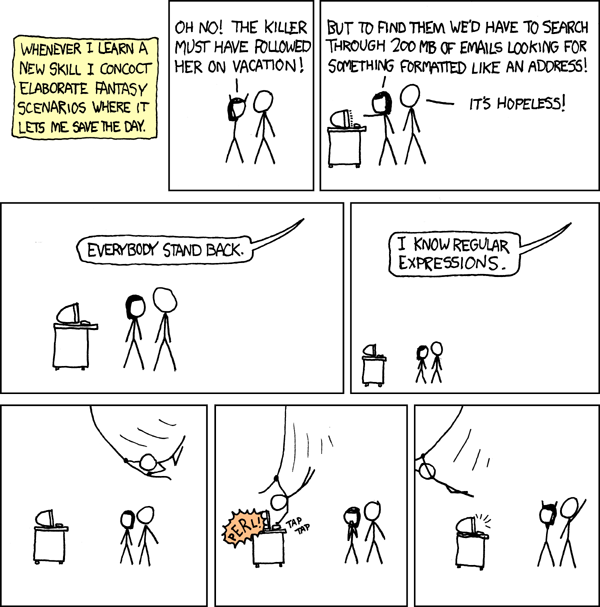
\includegraphics[width=\textwidth]{img/regular_expressions.png}
					
		\end{column}
		\begin{column}{0.53\textwidth}
		
		Une expression régulière est un motif qui correspond ou non à une chaîne de caractère donnée.
		%Randal Schwartz:
		%\textit{A \textit{regular expression} (…) is a template that either matches or doesn't match a given string. That is, there are an infinite number of possible text strings; a given pattern divides that infinite set in two groups: the ones that match, and the ones that don't. There's never any kinda-sorta-almost-up-to-here whishy-washy matching: either it matches or it doesn't.}
		
		\begin{block}{Ex.}
			\begin{itemize}
				\item \textbf{dates?} \textit{date} avec un ou sans \textit{s};
				\item \textbf{dat.*} \textit{dat} suivi de n'importe quoi ou de rien;
				\item \textbf{\textbackslash{}d\textbackslash{}d\textbackslash{}w\textbackslash{}w} 2 chiffres et 2 lettres.
			\end{itemize}
		\end{block}
		
		\end{column}
	\end{columns}
	
\end{frame}

% Outils plus spécialisés: ex., CQL; TXM, 
% Vers une interrogation personnalisée et fine des corpus: maîtrise d'XPath, SQL, etc.

\begin{frame}[fragile]
\frametitle{Quelques outils d'interrogation de données}
\framesubtitle{Langages de requêtes}

Des langages de requête spécifiques permettent d'interroger des données stockées selon un format spécifique.

	\begin{columns}
	\begin{column}{0.43\textwidth}
		\begin{block}{SQL}
			Interrogation de données stockées dans des bases relationnelles.
\begin{minted}{SQL}
SELECT * FROM table 
WHERE nom = 'JDupont'
\end{minted}
		\end{block}
	\begin{block}{SPARQL}
		Interrogation de données stockées en RDF.
	\end{block}
	\end{column}
	\begin{column}{0.55\textwidth}
		\begin{block}{XPath et XQuery}
			Interrogation de données stockées en XML
\begin{minted}[breaklines]{xml}
/TEI/text/body//persName[@ref = 'JDupont01']
\end{minted}
		\end{block}
	\begin{block}{CQL}
		Langage d'interrogation de corpus linguistique (\textit{Corpus Query Language}).\\
		\verb|[word='de.*'][]?[frpos='NP']|
	\end{block}
	
	\end{column}
\end{columns}


\end{frame}


\subsection{Méthodes quantitatives: des corrélations à la modélisation}

\begin{frame}{Résumer l'information avec des statistiques descriptives}

\begin{columns}
	\begin{column}{0.45\textwidth}
		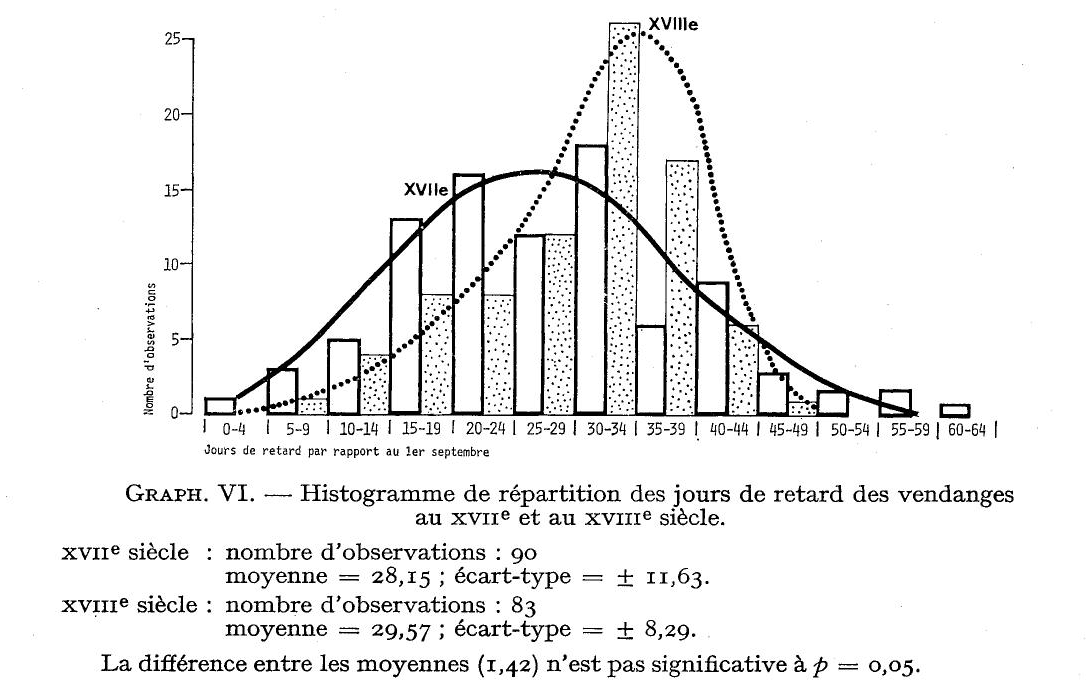
\includegraphics[width=1\textwidth]{img/ahess_0395-2649_1974_num_29_3_T1_0608_0000_006.png}
		
		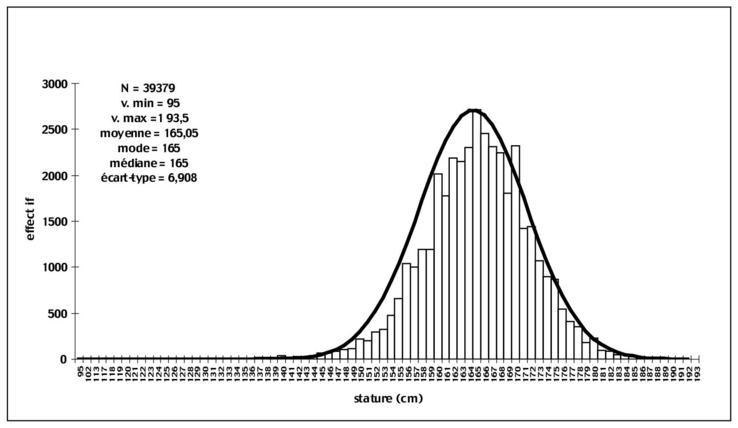
\includegraphics[width=1\textwidth]{img/Taille_conscrits.jpeg}
	\end{column}
	\begin{column}{0.45\textwidth}
		Comment aborder le vaste ensemble de données que l'on a constitué?
		
		Une approche \alert{statistique} permet de:
		\begin{itemize}
			\item résumer numériquement ou graphiquement une vaste quantité d'information;
			\item avoir des intuitions sur ses données;
			\item tester des hypothèses.
		\end{itemize}
		
	\end{column}
\end{columns}

\end{frame}

\begin{frame}{Détecter des corrélations}

\begin{columns}
	\begin{column}{0.45\textwidth}
		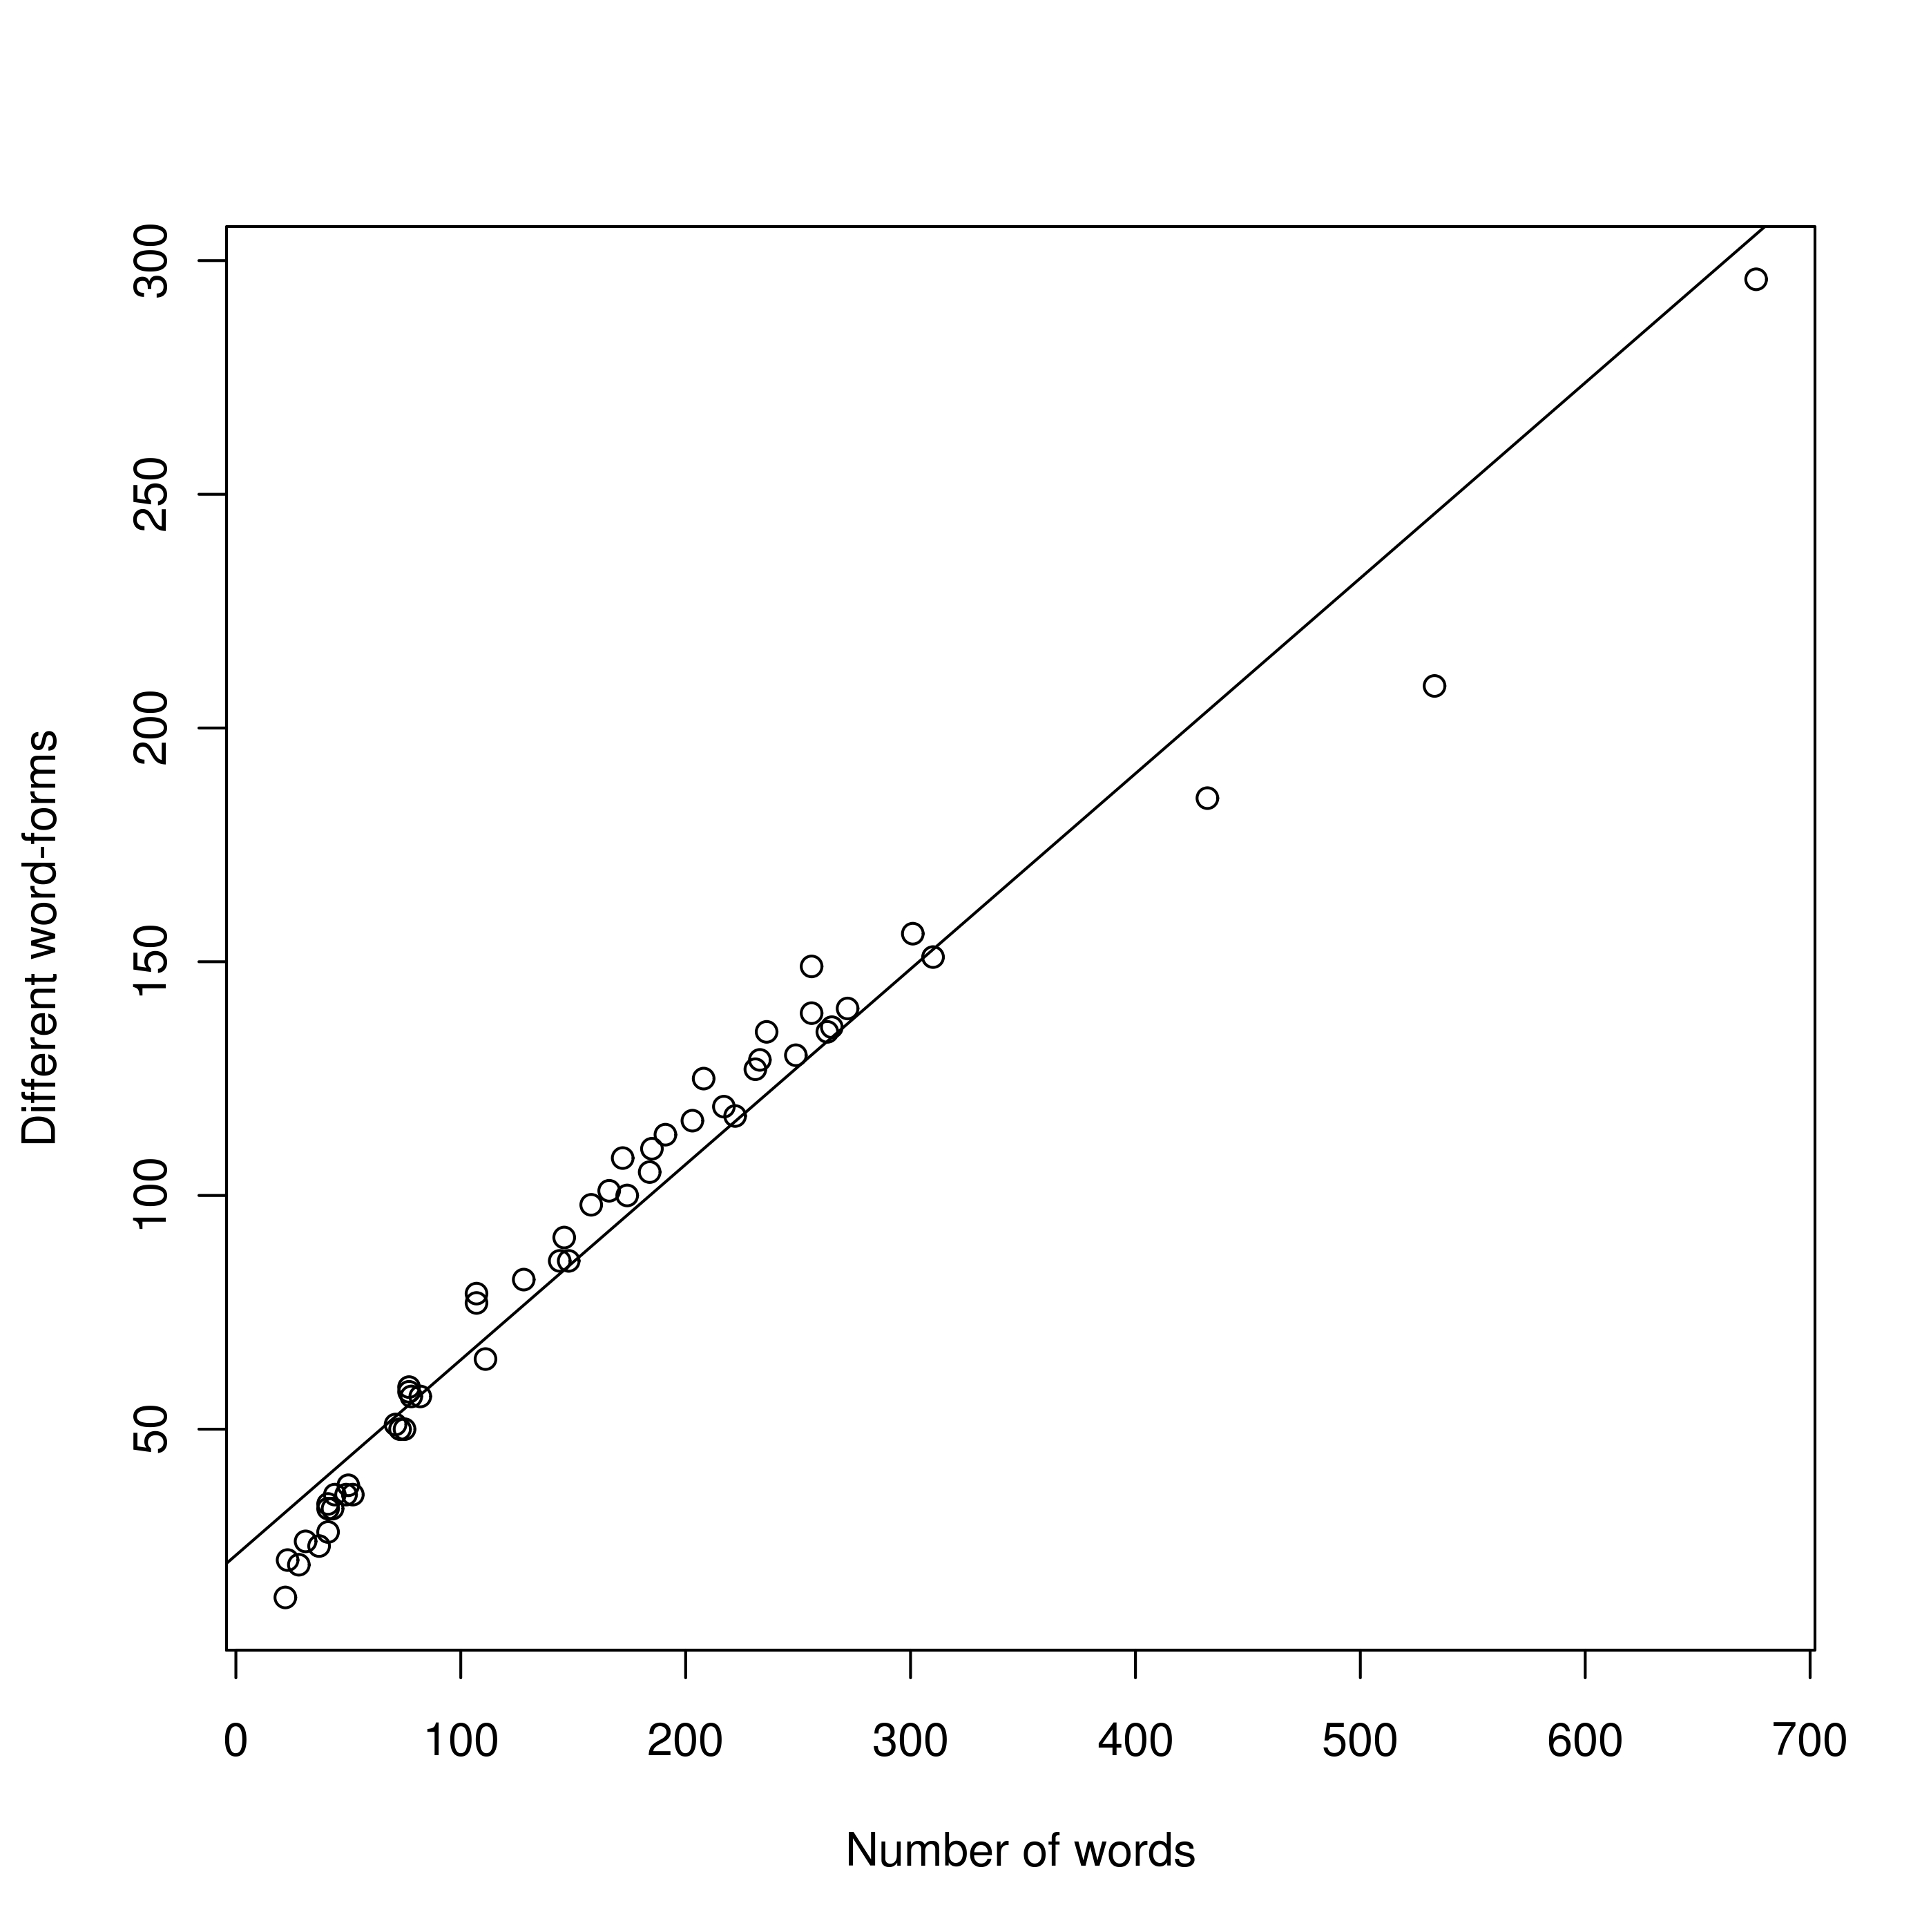
\includegraphics[width=\textwidth]{img/Regression_lineaire_richLex.jpg}
	\end{column}
	\begin{column}{0.45\textwidth}
		Identifier quand deux variables \alert{fonctionnent ensemble},\\
		et la \alert{significativité} par rapport au hasard.
		
	\end{column}
\end{columns}
\end{frame}

\begin{frame}{Écueils}

\begin{columns}
	\begin{column}{0.45\textwidth}
		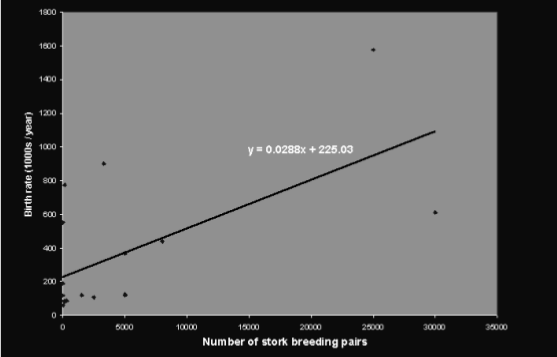
\includegraphics[width=\textwidth]{img/RM-storks-paper.png}
		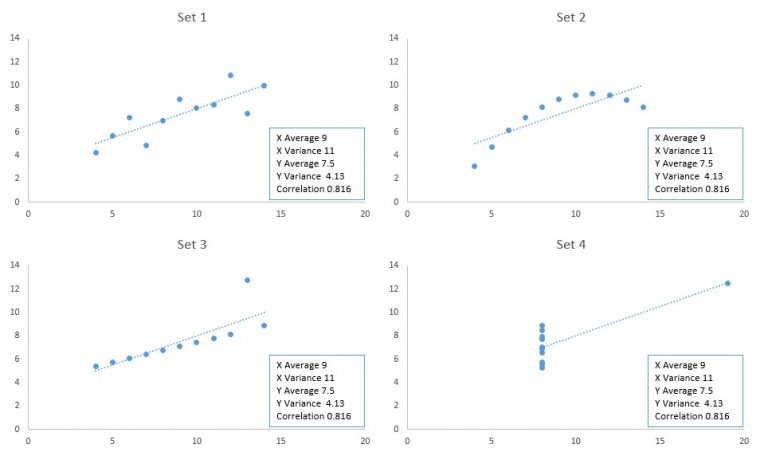
\includegraphics[width=\textwidth]{img/AnscombeQuarter.jpg}
	\end{column}
	\begin{column}{0.45\textwidth}
		\begin{block}{Cum hoc ergo propter hoc?}
			Corrélation n'est pas causalité.
		\end{block}
		\begin{block}{Qu'y a-t-il derrière une corrélation?}
			Des ``formes'' ou comportements très différents peuvent être caractérisés par le même niveau de corrélation.
		\end{block}
	\end{column}
\end{columns}

\end{frame}

\begin{frame}{Méthodes d'analyse et de visualisation}
	Une bonne partie des méthodes statistiques employées en HN trouvent leur origine dans d'autres champs: économétrie, biostatistiques,…
	
	Elles ont souvent une dimension très géométrique: calculs de distance, nuages de points, inertie…
\end{frame}

\begin{frame}{Régression}
\centering
		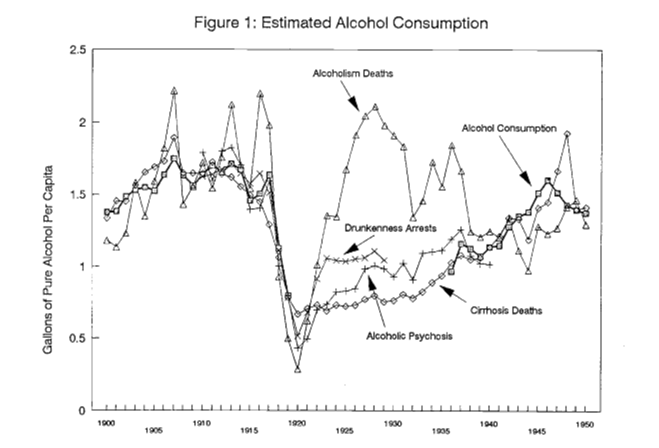
\includegraphics[width=0.9\textwidth]{img/Miron-proxy.png}

{\small J.A. Miron et J. Zwiebel, \textit{Alcohol
consumption during prohibition}, 1991.}

\end{frame}

\begin{frame}{Analyse par réduction de la dimensionnalité}

\begin{columns}
	\begin{column}{0.5\textwidth}
		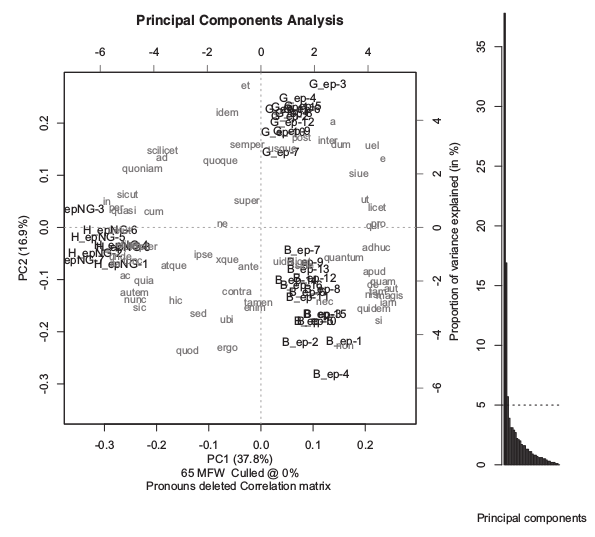
\includegraphics[width=\textwidth]{img/Kestemont_Hildegarde.png}
	
		{\small M. Kestemont \textit{et al.}, \textit{Collaborative authorship…}, 2015.}
	\end{column}
	\begin{column}{0.5\textwidth}
		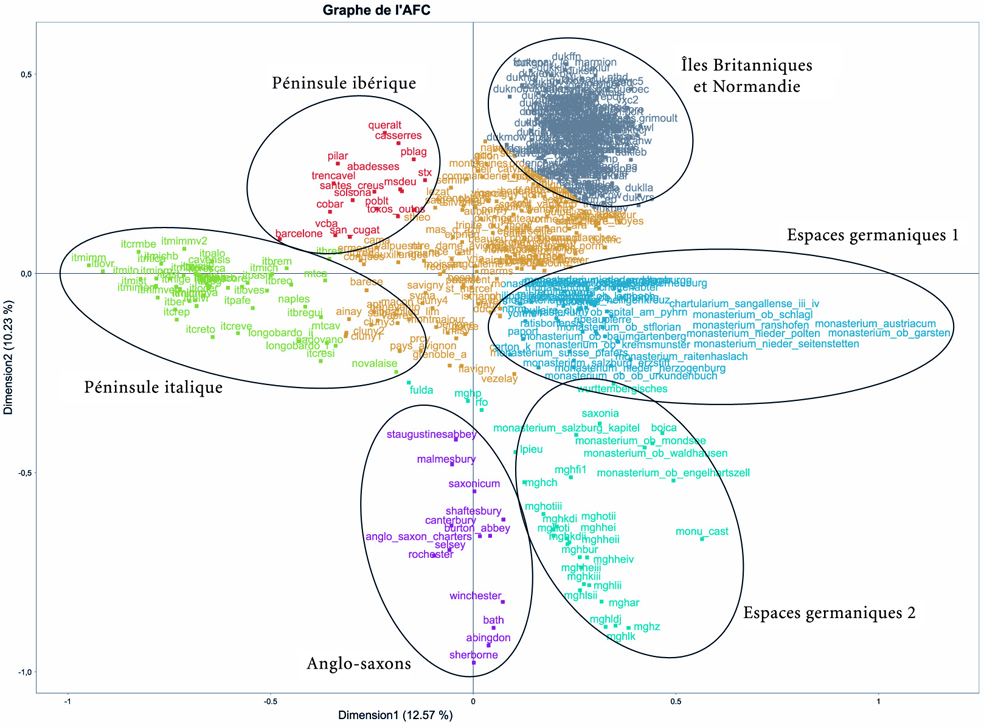
\includegraphics[width=\textwidth]{img/Perreaux_Chartes.jpg}
		
		{\small N. Perreaux, \textit{L'Écriture du  Monde…}, 2016.}
	\end{column}
\end{columns}

\end{frame}

\begin{frame}{Partitionnement de données}
		\begin{columns}
		\begin{column}{0.5\textwidth}
			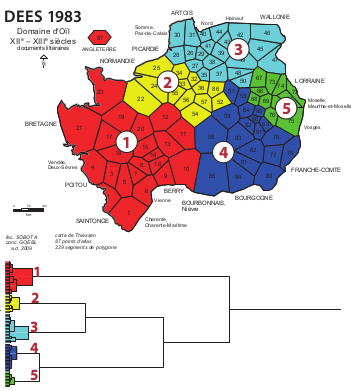
\includegraphics[width=\textwidth]{img/Goebl_2011_Medioevo_romanzo.png}
			
			{\small H. Goebl, \textit{L'aménagement scripturaire…}, 2011.}
		\end{column}
		\begin{column}{0.45\textwidth}
			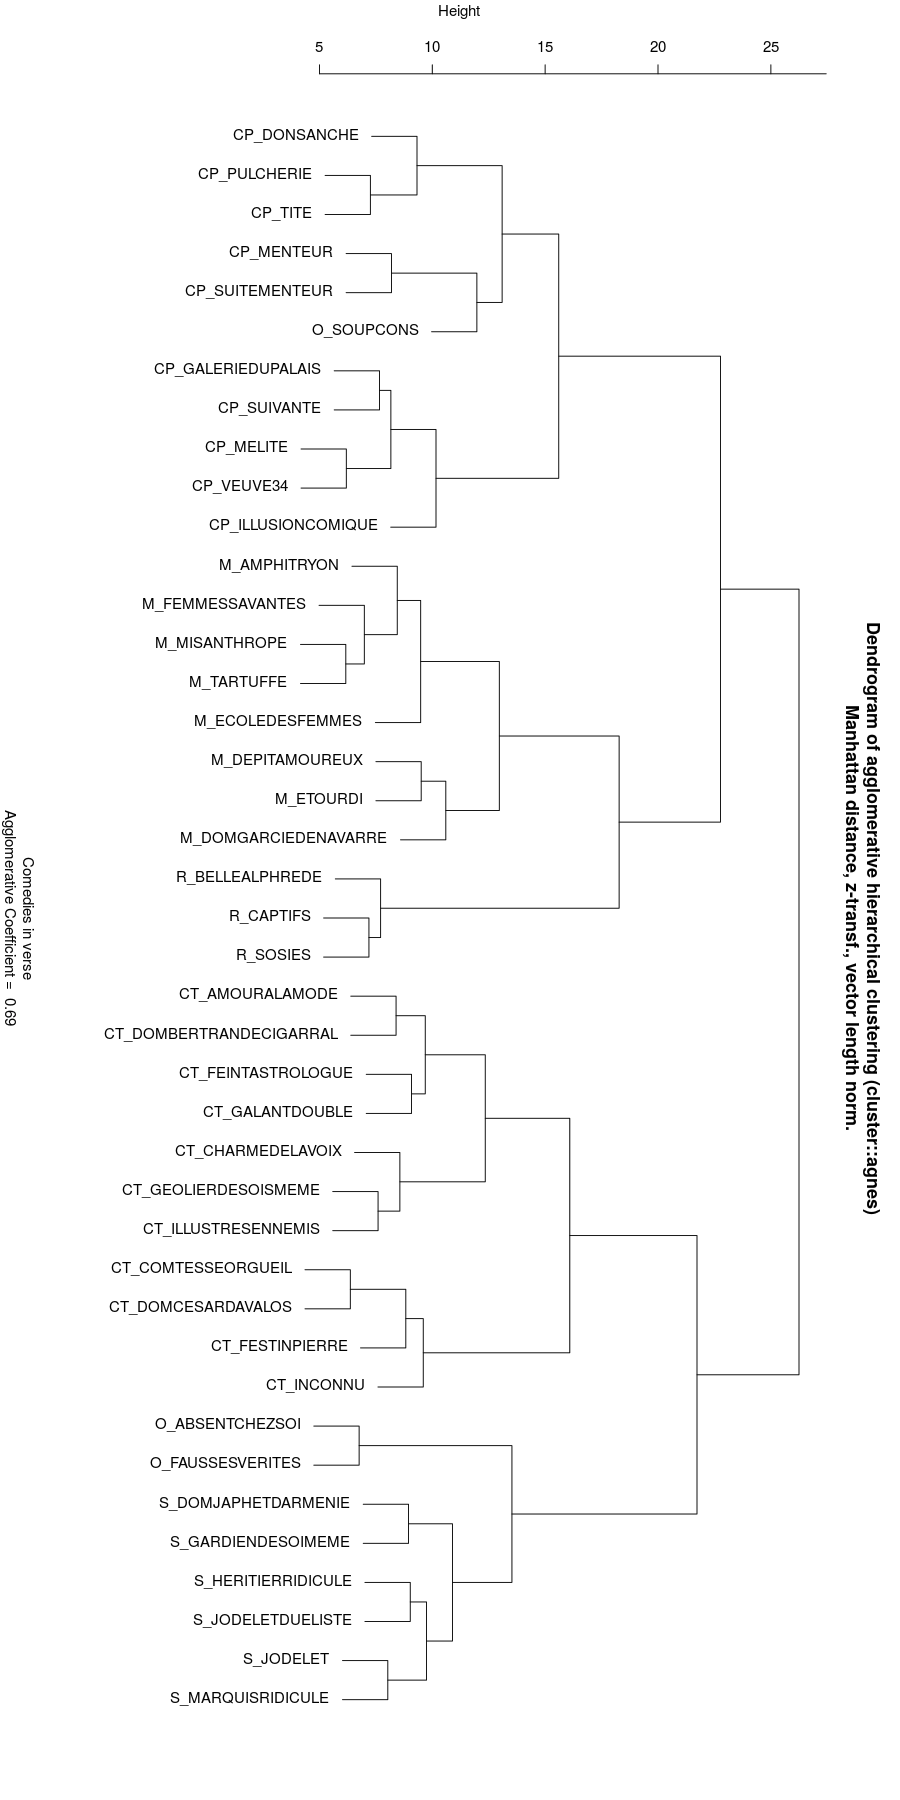
\includegraphics[width=0.9\textwidth]{img/CAH_Manhattan.png}
		\end{column}
	\end{columns}
\end{frame}

\begin{frame}{Quelques limites}
	\begin{columns}
		\begin{column}{0.5\textwidth}
			\begin{block}{Spécificités des données des SHS}
				\begin{itemize}
					\item données fragmentaires, manquantes;
					\item complexité;
					\item dimensionnalité;
					\item non linéarité (comme en physique).
				\end{itemize}
			\end{block}
		\end{column}
		\begin{column}{0.5\textwidth}
			\begin{block}{Des corrélations à la modélisation}
				Rendre compte des agents et de leurs comportements, de leurs interactions.
			\begin{itemize}
				\item systèmes dynamiques, multi-agents;
				\item transitions de phase?
			\end{itemize}
		Des interactions simples peuvent mener à beaucoup de complexité.
			\end{block}
		\end{column}
	\end{columns}
\end{frame}

\begin{frame}{Ex. modèle de Schelling et ségrégation urbaine}

\begin{columns}
	\begin{column}{0.5\textwidth}
		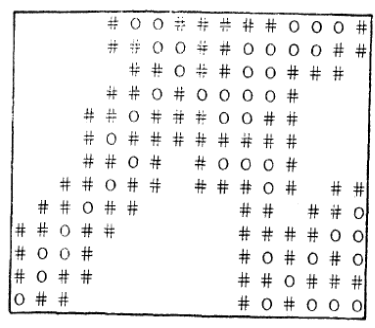
\includegraphics[width=\textwidth]{img/Schelling1.png}
		
		{\small T.C. Schelling, \textit{Jour. Math. Soc.} 1 (1971)}
	\end{column}
	\begin{column}{0.5\textwidth}
		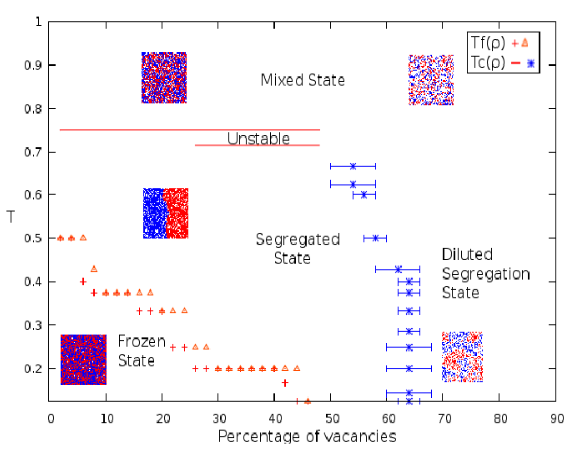
\includegraphics[width=\textwidth]{img/Schelling2.png}
		
		{\small Gauvin et al., \textit{European Physical Journal B}, 70, 293–304 (2009)}
	\end{column}
\end{columns}

\end{frame}

\begin{frame}{Ex. dynamique de population des manuscrits}

\begin{block}{}
	\begin{center}
		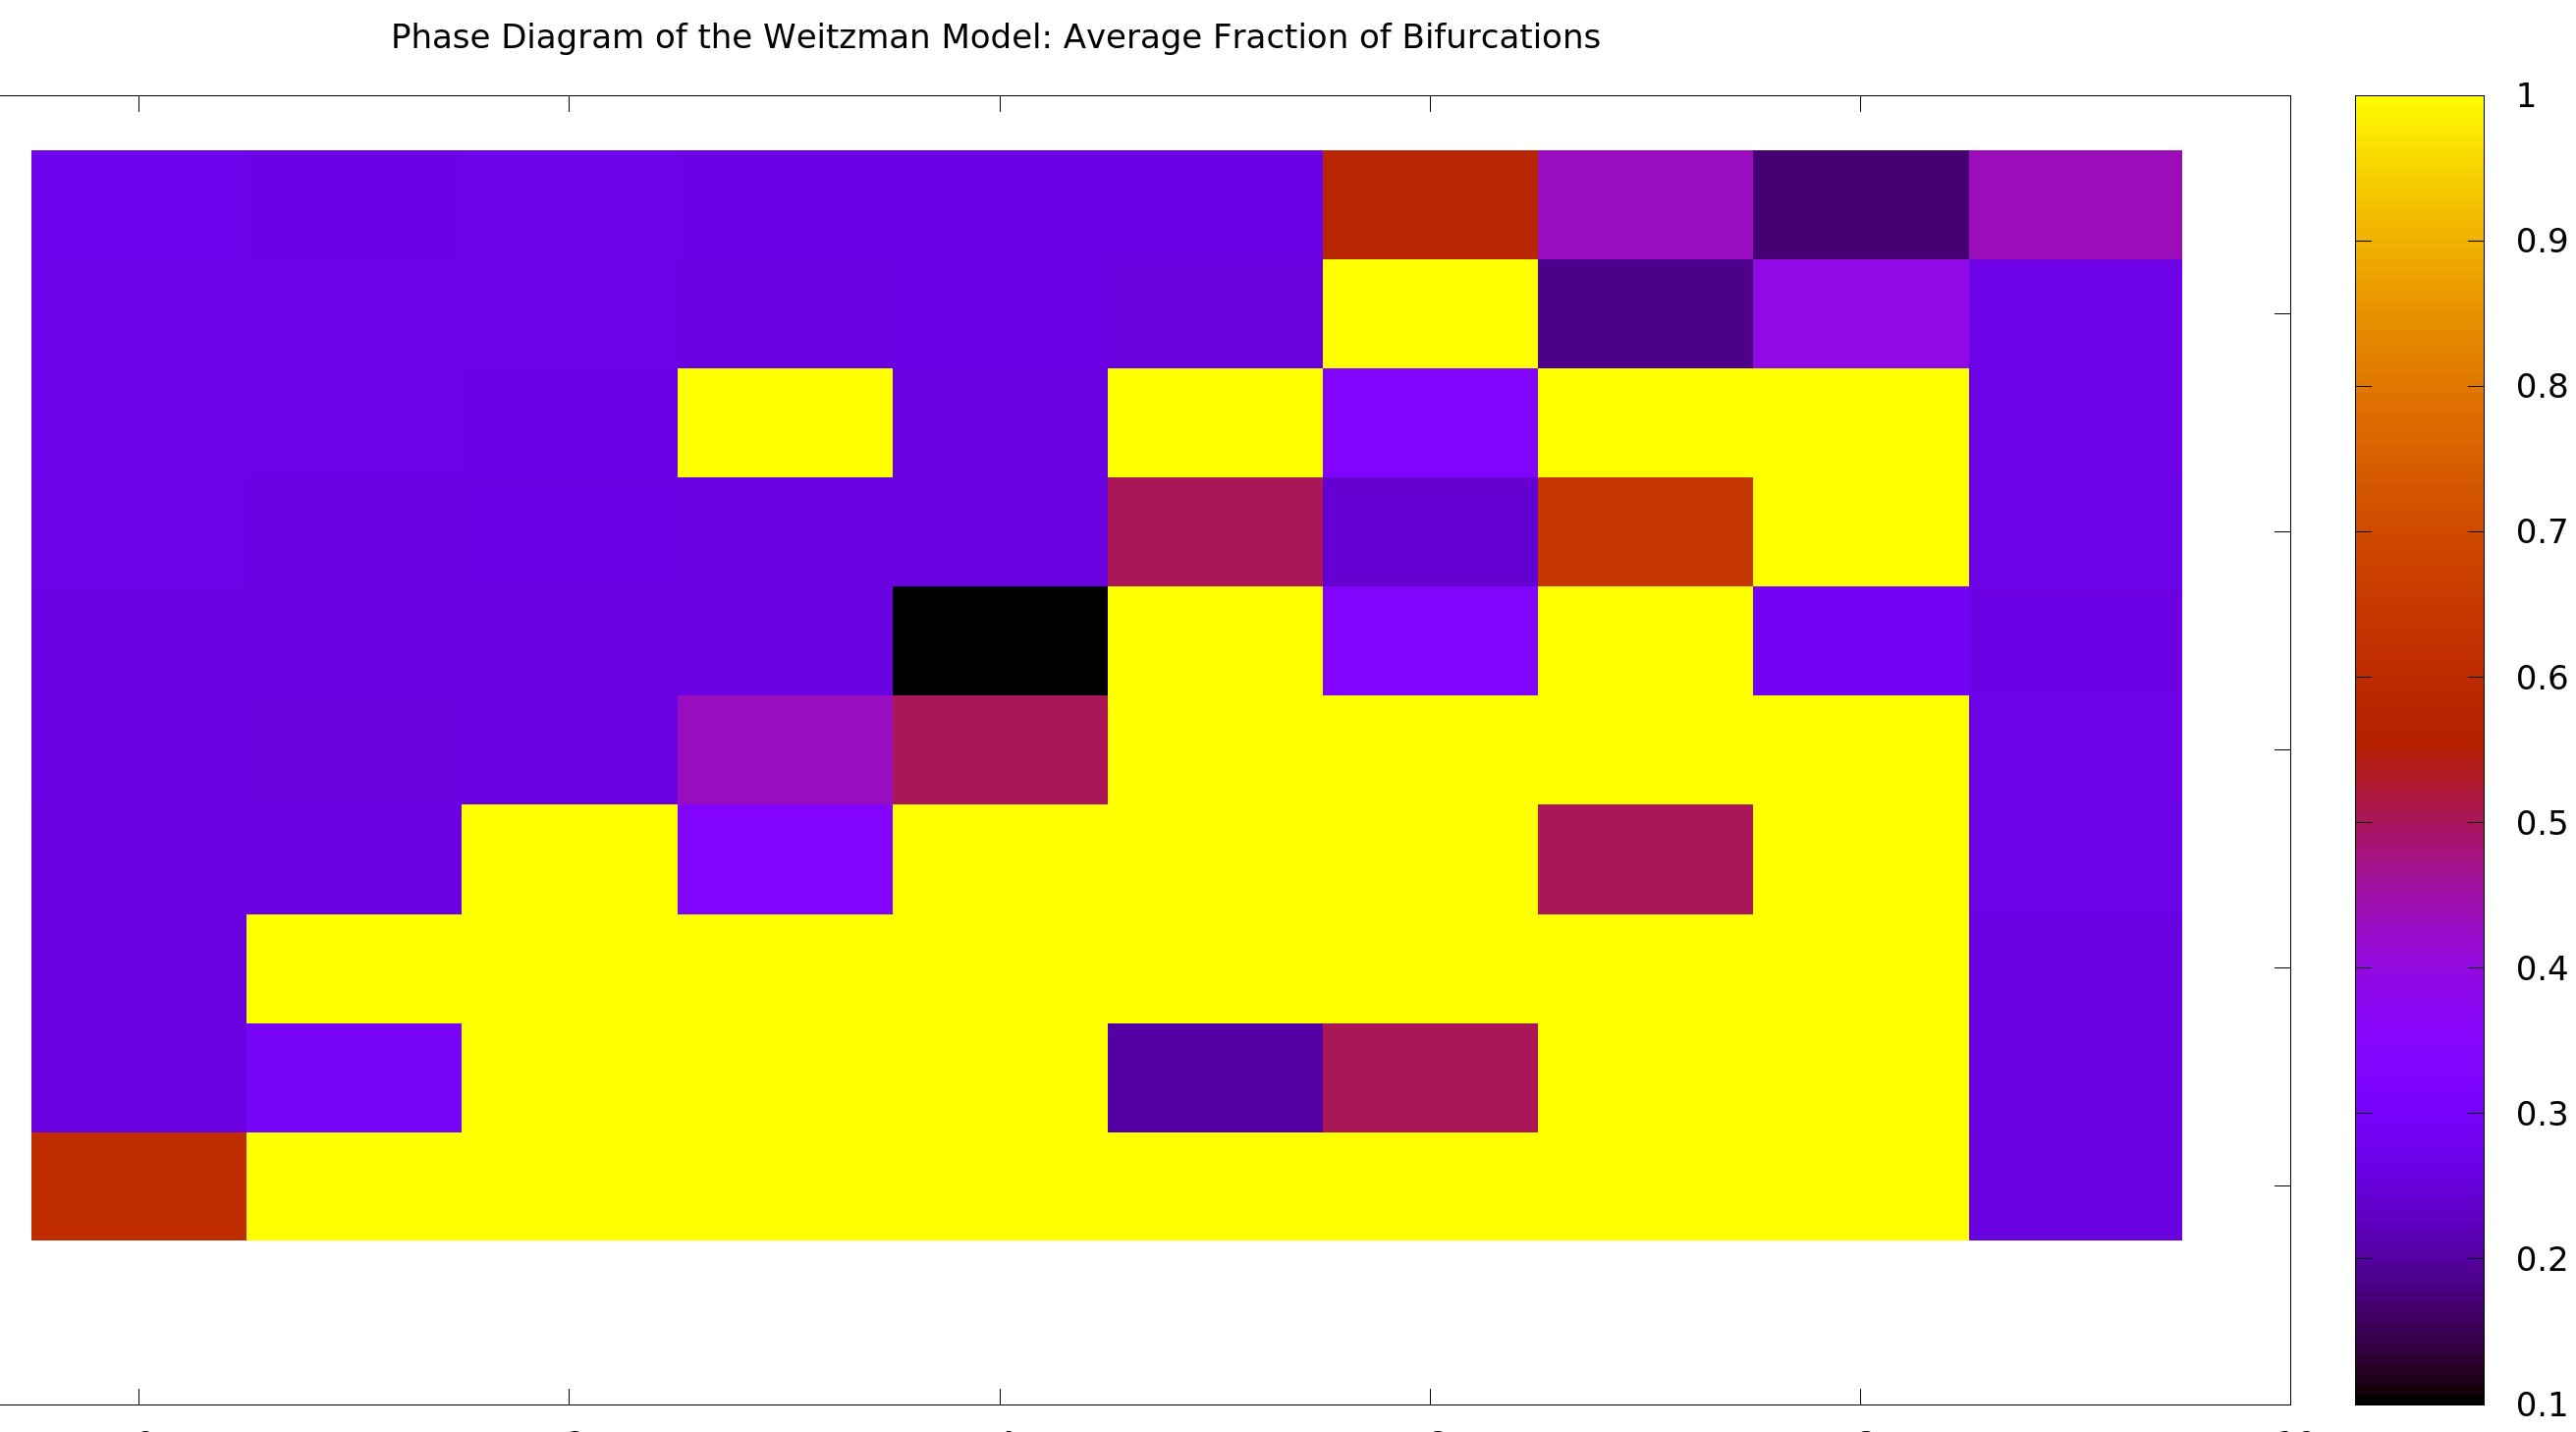
\includegraphics[scale=0.25]{img/PhDg01.jpeg}
	\end{center}
\end{block}
\begin{block}{}
	\begin{itemize}
		\item ``birth''/copy rate increases from bottom to top
		\item ``death''/decimation rate increases from left to right
		\item increments $=0.1$, from $0$ to $1$
		\item average fraction of bifurcations (over $10^2$ realisations, $500$ time steps each)
	\end{itemize}
\end{block}
\end{frame}


\subsection{Quelques outils particuliers} % des sciences sociales}

%SIG -> traité par E. Mermet

\begin{frame}{Ex. analyse de réseaux}
	
	\begin{columns}
		\begin{column}{0.5\textwidth}
			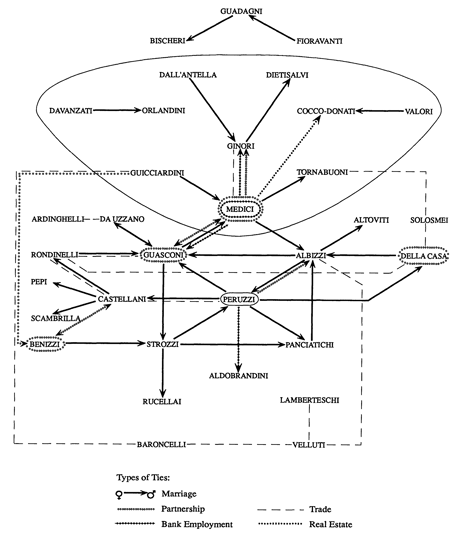
\includegraphics[width=\textwidth]{img/Padgett_Medici.png}
			
			{J.F. Padgett et Chr. K. Ansell, \textit{Robust Action…}, 1993.}
		\end{column}
		\begin{column}{0.5\textwidth}
		\begin{block}{Fondements théoriques}
			\begin{itemize}
				\item mathématiques: théorie des graphes, 
				\item sociaux: structure sociale vue comme un ensemble de relations entre individus.
			\end{itemize}
		\end{block}
	\begin{block}{Variété des applications}
		\begin{itemize}
			\item réseaux sociaux;
			\item réseaux de citations, emprunts, liens;
			\item réseaux de correspondance;
			\item etc.
		\end{itemize}
	\end{block}
	
		\end{column}
	\end{columns}
	
\end{frame}


\begin{frame}{En guise de conclusion provisoire…}
	
	\begin{block}{Pourquoi se lancer dans les humanités numériques?}
		\begin{enumerate}
			\item Parce que vous êtes le plus à même de le faire: vous connaissez votre sujet, vos données,…
			\item Parce qu'elles peuvent vous apporter un regard différent et de nouveaux résultats sur vos questions de recherche.
		\end{enumerate}
	\end{block}

\begin{block}{Un conseil}
	Apprendre à manier des logiciels spécialisés est nécessaire, mais, le meilleur investissement sur le long terme,
	\begin{enumerate}
		\item se familiariser avec un langage de programmation;
		\item acquérir des notions de stats et de mathématiques.
	\end{enumerate}
\end{block}	
	
\end{frame}


\end{document}
